%
% Concept leg
%

% !TEX root = ../main.tex

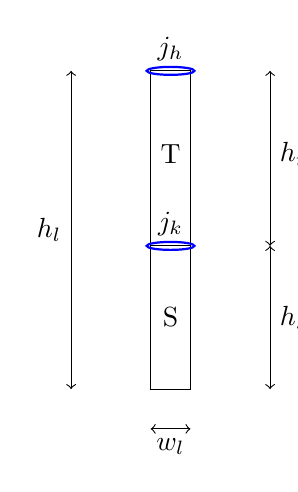
\begin{tikzpicture}[scale=\textwidth/12cm,trim right=(HS)]

  % Draw shank
  \coordinate (A) at (1,0);
  \coordinate (B) at (1.5,1.8);
  \draw (A) rectangle (B);
  \draw (1.25,0.9) node {S};

  % Draw thigh
  \coordinate (C) at (1,1.8);
  \coordinate (D) at (1.5,4);
  \draw (C) rectangle (D);
  \draw (1.25,2.95) node {T};

  % Draw hip joint
  \draw [blue,thick] (1.25,4) circle [x radius=0.3cm, y radius=0.05cm] node [text=black, above] {$j_h$};

  % Draw knee joint
  \draw [blue,thick] (1.25,1.8) circle [x radius=0.3cm, y radius=0.05cm] node [text=black, above] {$j_k$};

  % Draw height
  \coordinate (H0) at (0,0);
  \coordinate (HL) at (0,2);
  \coordinate (H1) at (0,4);
  \draw [<->] (H0) -- (HL) node [left] {$h_l$} -- (H1);

  % Draw height shank
  \coordinate (HS0) at (2.5,0);
  \coordinate (HS) at (2.5,0.9);
  \coordinate (HS1) at (2.5,1.8);
  \draw [<->] (HS0) -- (HS) node [text width=2cm ,right] {$h_s$} -- (HS1);

  % Draw height thigh
  \coordinate (HT0) at (2.5,1.8);
  \coordinate (HT) at (2.5,2.95);
  \coordinate (HT1) at (2.5,4);
  \draw [<->] (HT0) -- (HT) node [text width=2cm ,right] {$h_t$} -- (HT1);

  % Draw width
  \coordinate (W0) at (1,-0.5);
  \coordinate (WL) at (1.25,-0.5);
  \coordinate (W1) at (1.5,-0.5);
  \draw [<->] (W0) -- (WL) node [below] {$w_l$} -- (W1);

\end{tikzpicture}
